\section{Executive Summary}

This development period, we focused on implementing the \textbf{Customizable Automated Data Integration Pipeline}.
Approximately 90\% of this feature is completed, including:
\begin{itemize}
    \item Data aggregation and pipeline management systems
    \item An AI data mapping module for unified dataset creation
\end{itemize}

Remaining work involves completing the frontend-backend connection and refining the user interface for this module.

\section{Detailed Development Description}

\subsection{Overview}
The development scope focused on creating a data integration pipeline that automates the collection, processing, and unification of diverse data sources. Our objective was to implement an system capable of handling heterogeneous datasets from pipeline while minimizing manual configuration requirements. We adopted an iterative development approach, prioritizing core pipeline functionality before addressing user interface components.

\subsection{Key Classes and Modules Developed}

\begin{itemize}
    \item \textbf{pipeline/**}: This core module contains all components related to the Automated Data Integration Pipeline functionality
    \item \textbf{pipeline/ingestion/ingestors/mapping/mapping\_ingest.py}: Contains the AI mapping function that consolidates diverse data sources into a unified dataset structure
    \item \textbf{frontend/**}: Contains all user interface components, with specific emphasis on the pipeline configuration and monitoring interfaces
\end{itemize}

\subsection{Implementation Details and Challenges}
The data integration pipeline was implemented using a fastAPI combine with model fine-tuning on Vertex AI.
Here are lists of things we've developed

\begin{itemize}
    \item Data adaptor which consume data from API, File, and Scraping sources
    \item Data ingestor to help aggregate the data from each adaptor including AI ingestor module (AI data mapping module)
    \item Scheduling service to help manage pipeline
    \item Data store to save the pipeline configuration
    \item UI interface for pipeline service
\end{itemize}

We faced several challenges. First, the scraping adapter doesn’t work on Windows right now. Second, the scheduling service was poorly designed, which caused many problems and now needs to be redesigned. We also had trouble building stable data connectors for different data sources. It was hard to create a smart mapping system that could understand how different data formats are related. Changing the data while keeping it correct was another challenge. Finally, making sure the system can handle a large amount of data was also difficult.

\subsection{Screenshots}

\begin{figure}[H]
    \centering
    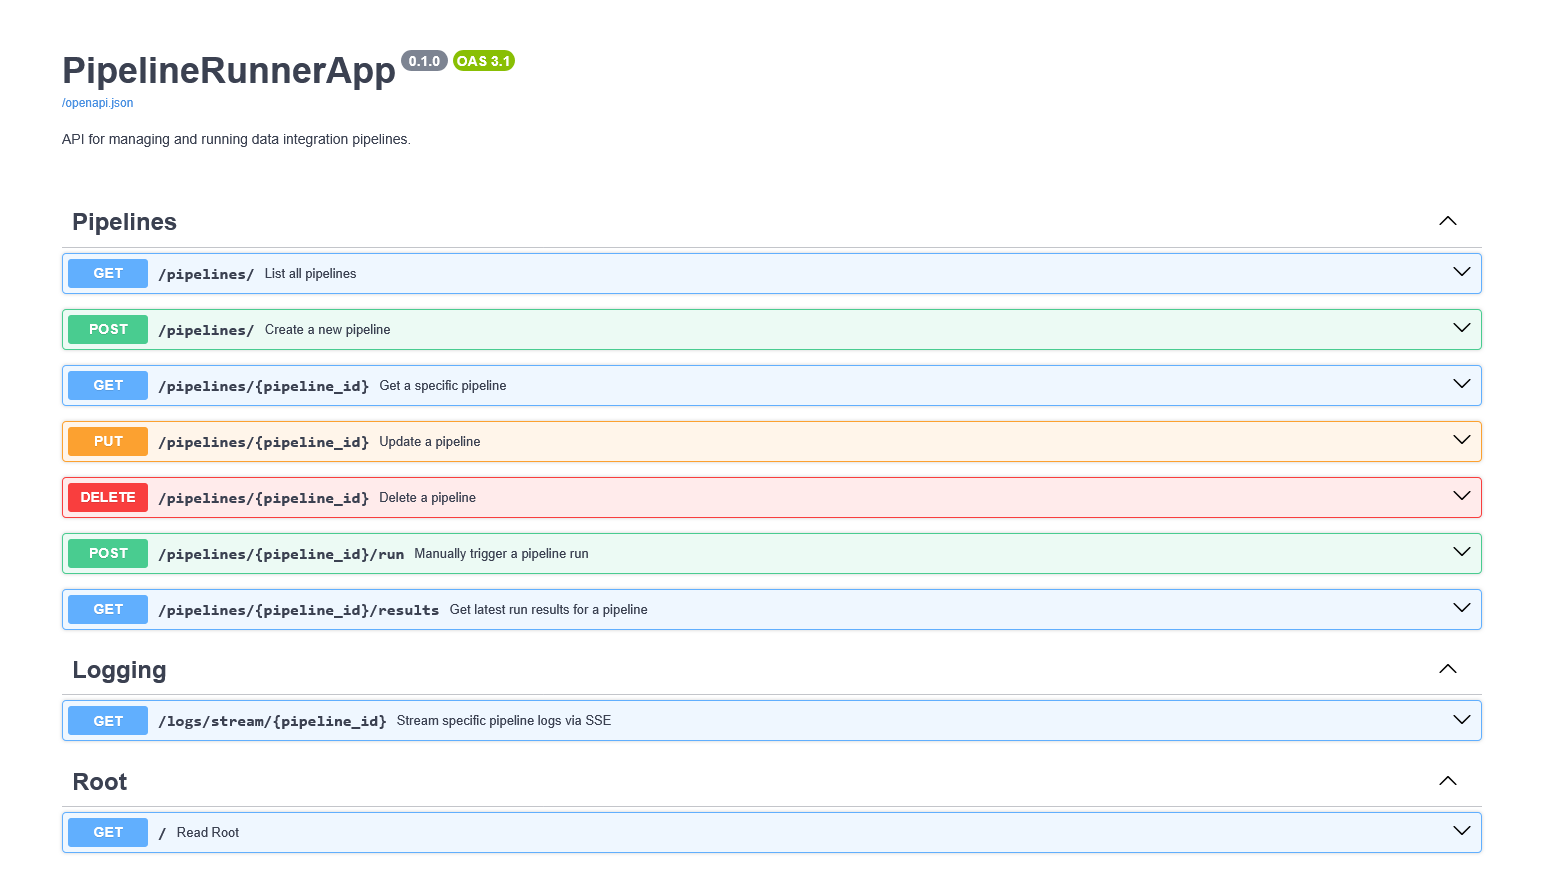
\includegraphics[width=0.8\textwidth]{assets/api-doc.png}
    \caption{API documentation interface for pipeline management endpoints, providing comprehensive testing capabilities for backend functionality}
    \label{fig:api-doc}
\end{figure}

\begin{figure}[H]
    \centering
    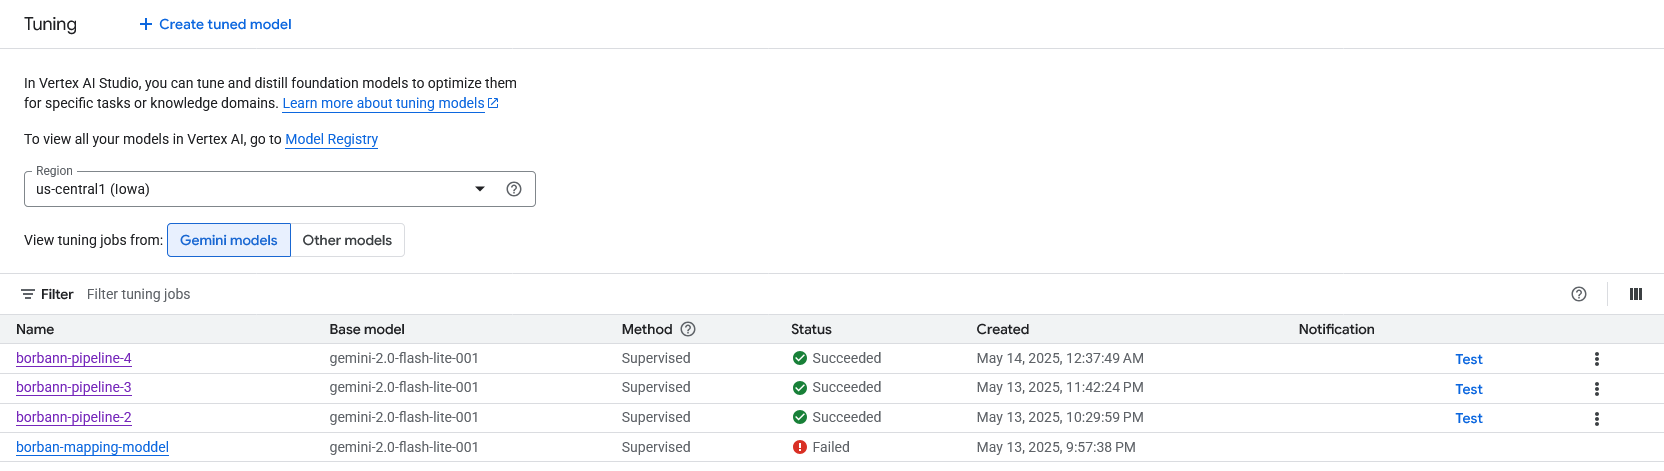
\includegraphics[width=0.8\textwidth]{assets/vertex/model-versioning.png}
    \caption{Data Mapping LLM models with multiple versions}
    \label{fig:model-versioning}
\end{figure}

Figure 2 display versions of data schema apping model that we fine-tune on Vertex AI platform.

\begin{figure}[H]
    \centering
    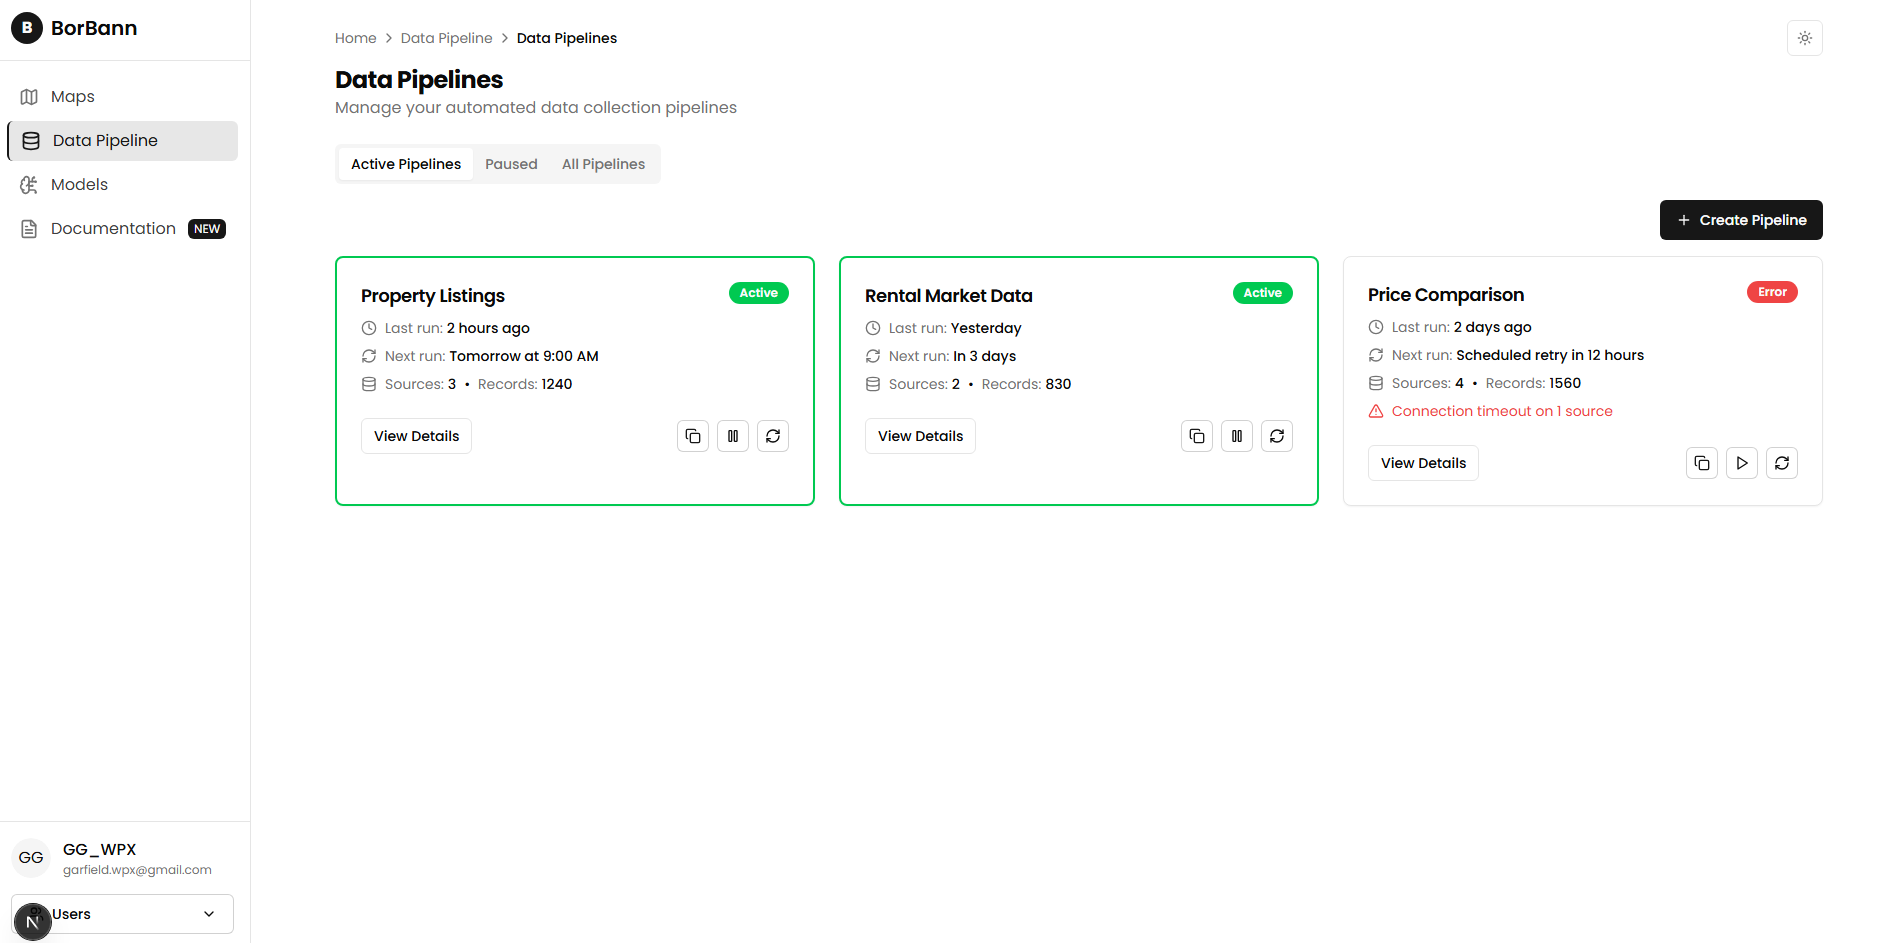
\includegraphics[width=0.8\textwidth]{assets/pipeline.png}
    \caption{Pipeline status UI interface}
    \label{fig:pipeline-status-ui}
\end{figure}

Figure 3 is an example of UI interface we have been developed along with the pipeline backend service.


\subsection{Experimental Results}

Performance metrics are based on 2 metrics:
        \begin{itemize}
            \item \textbf{JSON Syntactic Validity}: Parse the output string and check for validity.
            \item \textbf{Pydantic Schema Conformance}: Check with pre-defined pydantic schema to ensure that it output the desire data scheme.
        \end{itemize}

There is a problem on the training data so conformance scores are low, we will fix it.


\begin{table}[htbp]
    \centering
    \caption{Model Validation Metrics}
    \label{tab:model_comparison}
    \begin{tabular}{llc}
        \toprule
        \textbf{Model Version} & \textbf{Metric} & \textbf{Value (\%)} \\
        \midrule
        \textbf{BORBANN\_PIPELINE\_2} 
            & JSON Syntactic Validity & 91.67\% \\
            & Pydantic Schema Conformance & 63.64\% \\
        \midrule
        \textbf{BORBANN\_PIPELINE\_3} 
            & JSON Syntactic Validity & 100.00\% \\
            & Pydantic Schema Conformance & 0.00\% \\
        \midrule
        \textbf{BORBANN\_PIPELINE\_4} 
            & JSON Syntactic Validity & 100.00\% \\
            & Pydantic Schema Conformance & 0.00\% \\
        \bottomrule
    \end{tabular}
\end{table}

\subsection{Datasets Acquired or Used}

We mainly based on two sources; data from implemented pipeline service and generated data from LLM

\begin{itemize}
    \item \textbf{Collected from pipeline service} -- Combine the data output from pipeline with specific prompt to create user role and define the target canonical dataset for model role
    \item \textbf{Generate with Gemini 2.5 Flash Preview 04-17 with this prompt} -- Craft prompt to more synthetic datas and cover more cases
\end{itemize}

\subsection{Updated Development Plan}

Here is the updated gantt chart

\begin{figure}[H]
    \centering
    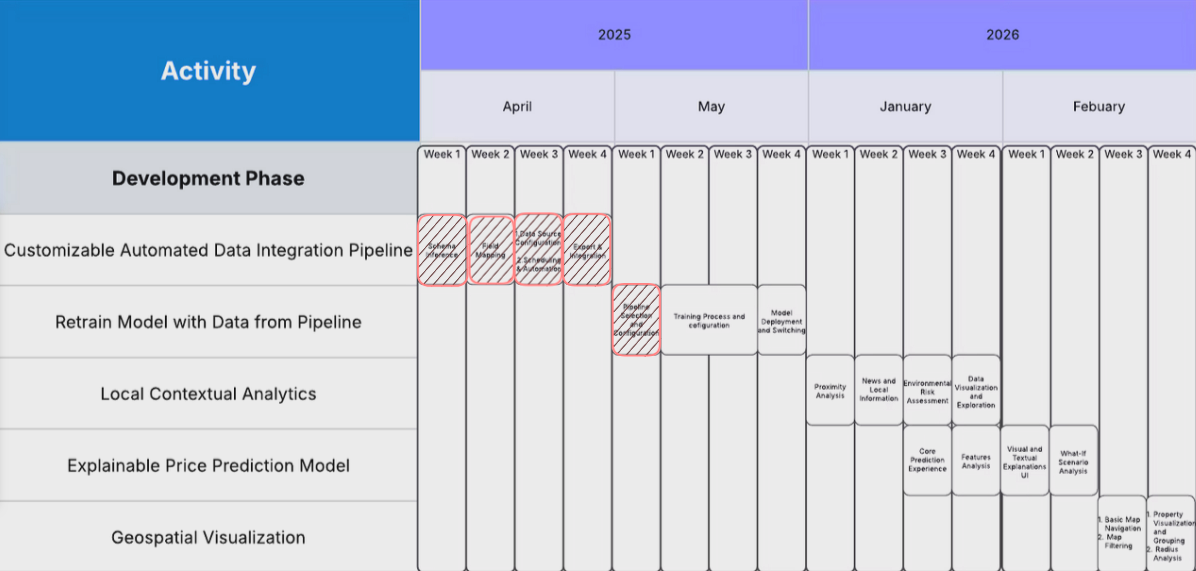
\includegraphics[width=0.8\textwidth]{assets/gant.png}
    \caption{Gantt Chart}
    \label{fig:gantt}
\end{figure}


\subsection{Self-evaluation}

I think this pass month we have done a lot of things such as system design and UI design, our progress is faster on the frontend side
and we think that on the backend is a bit slower due to challenges such as integrity of data in pipeline, so we need to redesign the pipeline service many times.
Also, we have a bit problem on the scheduling of pipeline too, so we need to rewrite it too due to bad design.

Overall, We think that we need to work harder if we want to finish this project in time with good quality.